
\documentclass{article}
\usepackage{cite}
\usepackage{amsmath,amssymb,amsfonts}
\usepackage{algorithmic}
\usepackage{graphicx}
\usepackage{textcomp}
\usepackage{xcolor}
\usepackage{float}
%\def\BibTeX{{\rm B\kern-.05em{\sc i\kern-.025em b}\kern-.08em
%		T\kern-.1667em\lower.7ex\hbox{E}\kern-.125emX}}
	
\begin{document}
	
	\title{Parallel Genetic Programming}
	
	\author{Abiyaz Chowdhury \and Allen Kim}
	
	\maketitle
	
	\begin{abstract}
Genetic programming is a technique in the field of genetic algorithms that evolve computer programs themselves. Programs are encoded in some computational representation that are then run through the standard genetic operations (selection, crossover, mutation). However, the computational cost to train genetic programs grows rapidly as the complexity of the problem increases. We aim to implement a highly parallel version of genetic programming that will scale efficiently.
	\end{abstract}
	
	\section{Introduction}
	Genetic algorithms have primarily seen use in optimizing numerical parameters. However, genetic programming has not seen as much mainstream use in the past due to its severe computational costs. Genetic programming aims to evolve the computer program themselves over time rather than various function parameters \cite{b1}. By having programs themselves be the population, genetic programming ultimately aims to have computer-generated programs that show distinct characteristics from human written programs and ideally, efficient as well.
	
	The main problem with genetic programming is the fact that in practice, it is only able to solve small problems. The sheer number of possible programs that exist makes it difficult to even create simple programs. However, with the growth in modern computing power and the use of parallelism, genetic programming is beginning to seem more practical.
	
	\section{Prior Work}
	
	One main topic in prior work in genetic programming deals with how to represent the programs themselves structurally. The simplest idea was to use a forest of parse trees since compilers are used to dealing with such structures for programs, but they tend to be much slower to analyze. Other data structures such as directed acyclic graphs \cite{b2} were later proposed to allow for greater efficiency, but we focused on parallel distributed genetic programming (PDGP) \cite{b3}. 
	
	In PDGP, programs are encoded as grids in which each node can be non-terminal or terminal. Non-terminal nodes represent different functions that take in other nodes as arguments while terminal nodes represent the input to the program. There are many variations to the grid, but we chose one of the simplest representations. Akin to a feed forward neural network, we considered grids that had connective edge between adjacent layers. Thus, our programs would propagate values upward from bottom to top through a series of nodes. This was still an efficient representation as nodes can be reused by the layers above, but was also simple enough to understand and implement. With the identity node, any grid could be represented in this way given sufficient rows and columns.
	
	Regarding the parallel implementations of genetic programming, most prior work splits up the population among the processors and evaluate fitness in parallel \cite{b4}. We aimed to implement these core ideas in our program as well.
	
	
	\section{Overview}
	For our project, we implemented a parallelized version of PDGP, which was built to solve arbitrary combinatorial circuit problems. We allow the use of AND, OR, NOT, NAND, NOR, and I (identity) as our non-terminals. We also use $x_1$ to $x_n$ for our input. Given a function we want to learn, we use our program to find circuits that can solve it. We test our program on solving XOR as well as solving the even-3 parity problem. 
	
	Regarding parallelization, we experimented with parallelizing different aspects of the project. We found that for small grids, parallelizing the tasks related to computing on a single grid was not efficient. Thus, most of our parallelization was in the genetic programming itself, which we discuss in the implementation section.
	
	\section{Description of Implementation}

	\subsection{Random Graph Generation}
	To initialize the graph, we assume that we are given a set width and height for our grid. Then, we randomly fill the grid with non-terminal and terminal nodes randomly. We do place certain constraints, however. The bottom row of the grid are always restricted to be terminals while the output node at the top is always restricted to be non-terminal. This is to ensure that every grid corresponds to a valid program. By default, each node is inactive, but after initializing, we mark every node connected to the output as active. An example is shown in Figure \ref{sample1}.
	
	\begin{figure*}
		\centering
		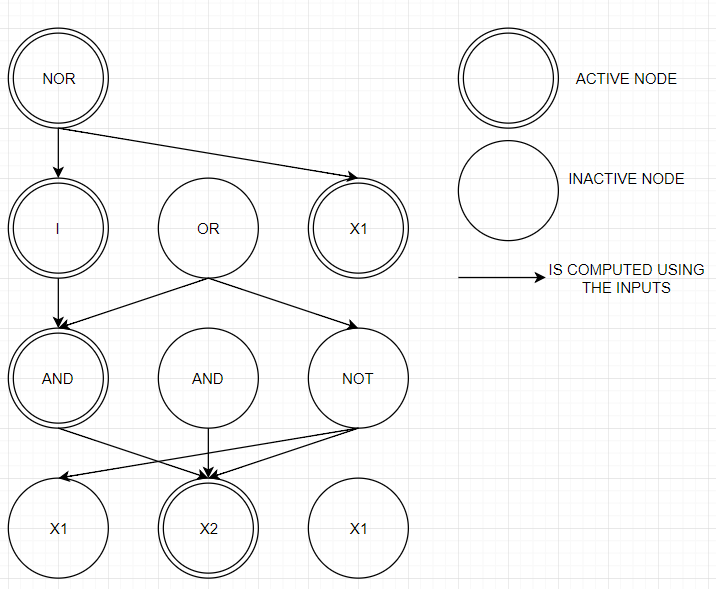
\includegraphics[width=\textwidth]{sample1.png}
		\caption{Example random grid}
		\label{sample1}
	\end{figure*}
	
	For our random number generator, we use a variant of XOR shifting pseudo random number generators, which run much faster than the rand function in the standard library. This is important to optimize the speed in which our populations are generated.
	
	For larger grids, it may potentially be faster to parallelize the generation of the population, but for our case, the grids were small enough that benefits were not seen in adding more processors.

	\subsection{Evaluation and Fitness}
	For our evaluation, we compute the values for the output bottom up in the grid. At each node, we consider only the active nodes and cache the temporary value for the output as we move up. For fitness, we use the Hamming distance from the truth table. Since we chose to maximize fitness for our population, we subtract the Hamming distance from the total possible outputs, which is exponential in the input.
	
	\subsection{Genetic Operators}
	\subsubsection{Crossover}
	For crossover, there are many variations discussed in Poli's work on PDGP, but we chose to implement the one that seemed most effective and simplest to implement: sub-sub graph active-active node. In this version of crossover, we first randomly select an active node from the one graph and a random active node from the second graph. Then, we copy the subgraph rooted at the first node over to the second node. We prune off any nodes that may extend beyond the graph as well. An example of this is shown in Figures \ref{sample2} and \ref{sample3}.
	\begin{figure*}[h!]
		\centering
		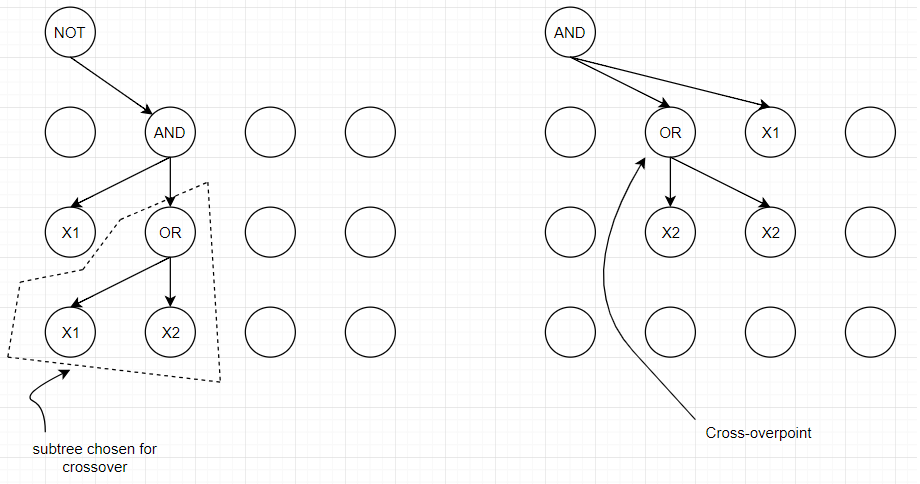
\includegraphics[width=\textwidth]{sample2.png}
		\caption{Before Crossover}
		\label{sample2}
	\end{figure*}
	\begin{figure*}[h!]
	\centering
	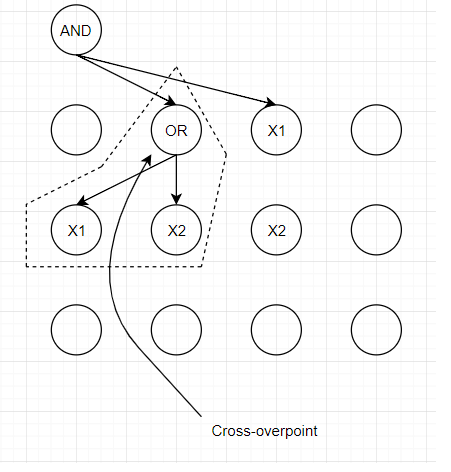
\includegraphics[scale=1]{sample3.png}
	\caption{After Crossover}
	\label{sample3}
\end{figure*}
	
	
	\subsubsection{Mutation}
	We consider three forms of mutations: global, link, and node. The first two are discussed in Poli’s original work, but the third form was not used. We also implemented it to see if it had any positive effect.
	\begin{itemize}
		\item Global mutation injects a random subgraph at a random active node in the candidate graph. We implemented this by conducting crossover with a randomly generated graph.
		\begin{figure*}
			\centering
			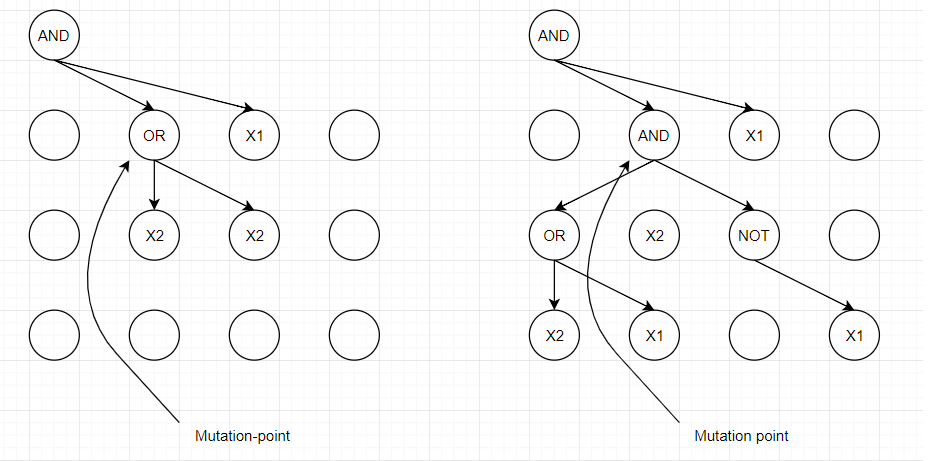
\includegraphics[width=\textwidth]{sample4.png}
			\caption{Global Mutation}
			\label{sample4}
		\end{figure*}
		
		\item Link mutation randomly changes an edge in the grid to point to a random node below it.
		\begin{figure*}
			\centering
			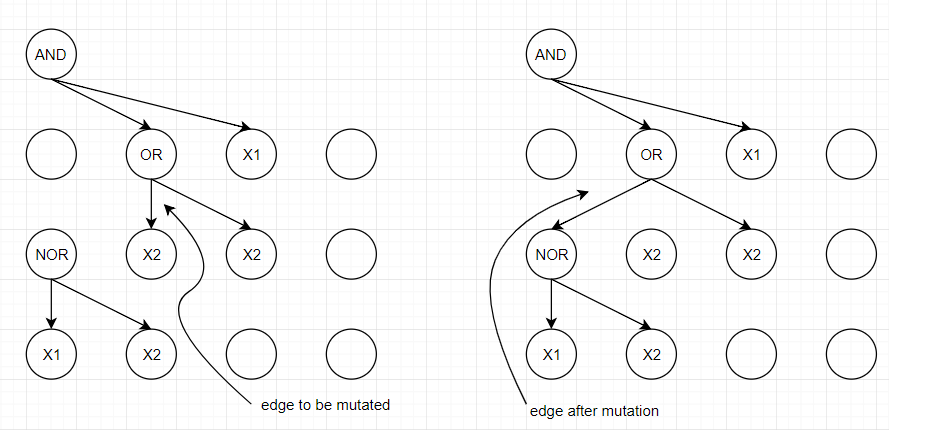
\includegraphics[width=\textwidth]{sample5.png}
			\caption{Link Mutation}
			\label{sample5}
		\end{figure*}	
	
		\item Node mutation randomly changes a node in the grid to become terminal or non-terminal and then, randomly assigns a new function or value to the node.
		
		\begin{figure*}
			\centering
			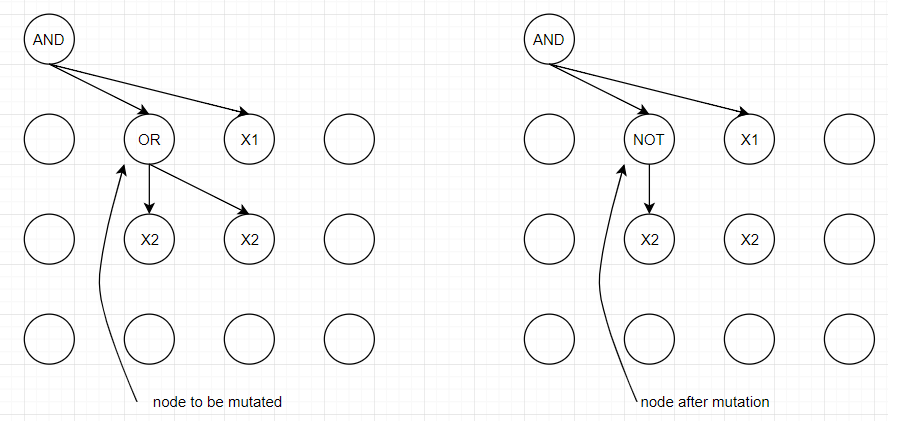
\includegraphics[width=\textwidth]{sample6.png}
			\caption{Node Mutation}
			\label{sample6}
		\end{figure*}
		
	\end{itemize}
	\subsubsection{Selection}
	For selection, we use tournament selection where the size of tournament is a parameter to the program. In tournament selection, we are given a number of participants, say $k$, and we randomly sample $k$ candidates from the current population. The one with the highest fitness from this set is selected. By varying the tournament size, one can control the selection pressure. If the tournament size is small, then candidates with lower fitness are more likely to survive whereas if the tournament gets larger, then there are more and more possibilities for stronger candidates to go through.
	
	\subsection{Run of a single generation}
For a single generation, we run the following steps:
\begin{enumerate}
\item Run selection twice to find candidates for both parents.
\item With some probability, conduct crossover to create a child grid.
\item With some probability, run global mutation on the child.
\item With some probability, run link mutation on the child.
\item With some probability, run node mutation on the child.
\item Add the child to the new population and repeat steps 1 to 5 until population is full.
\end{enumerate}

	\subsection{Multi-start Evaluation}
	Since genetic programming is not guaranteed to converge to the global best, we also employ a simple technique to try and initialize and run our programs with different seeds. We then take the best fit across all of these programs. This is easily parallelizable since each genetic program can be run independently from one another. 
	
	\section{Analysis}
	We now conduct a running time analysis of our genetic program.
	
	To generalize, we use the following variables in our program: $x$ for the number of inputs, $b$ for the number of bits per input, $m\times n$ grid size, $\alpha$ for the largest arity out of the non-terminals, $S$ for population size, $k$ for tournament size, $G$ for number of generations, and $T$ for the number of multi-starts.
	\begin{align*}
	\texttt{eval} &= O(mnA) \\
	\texttt{fitness} &= O(mnA2^{bx})\\
	\texttt{generate-graph} &= O(mnA)\\
	\texttt{evaluate-fitness} &= O(SmnA2^{bx})\\
	\texttt{initialize-pop} &= O(SmnA + SmnA2^{bx})\\
	\texttt{crossover} &= O(mnA)\\
	\texttt{global-mutation} &= O(mnA)\\
	\texttt{link-mutation} &= O(mnA)\\
	\texttt{node-mutation} &= O(mnA)\\
	\texttt{selection} &= O(k) \\
	\texttt{next-gen} &= O(S(2k + 4mnA) + SmnA2^{bx}) \\
	\texttt{run} &= O(G(S(2k + 4mnA) + SmnA2^{bx})) \\
	\texttt{run-ensemble} &= O(T(G(S(2k + 4mnA) + SmnA2^{bx})))
	\end{align*}
	We now provide a brief description of each function:
	\begin{align*}
	\texttt{eval} &= \text{evaluate output given input values for a single grid} \\
	\texttt{fitness} &= \text{compute Hamming distance fitness of a grid}\\
	\texttt{generate-graph} &= \text{initialize a random grid}\\
	\texttt{evaluate-fitness} &= \text{evaluate fitness for each member of population}\\
	\texttt{initialize-pop} &= \text{generate grids for each individual in population size}\\
	\texttt{crossover} &= \text{crossover as described prior}\\
	\texttt{global-mutation} &= \text{global mutation as described prior}\\
	\texttt{link-mutation} &= \text{link mutation as described prior}\\
	\texttt{node-mutation} &= \text{node mutation as described prior}\\
	\texttt{selection} &= \text{selection as described prior} \\
	\texttt{next-gen} &= \text{single run as described prior} \\
	\texttt{run} &= \text{runs next gen for certain number of generations} \\
	\texttt{run-ensemble} &= \text{run multi-start number of instances}
	\end{align*}

	Simplifying \texttt{run-ensemble}, since $k$ is upper bounded by $S$, we get that it takes $$T_1 = O(TGSmnA2^{bx})$$ With parallelism, we get that $$T_\infty = O(GmA\log T \log S)$$
	The logs follow from the fact that finding the maximum over an array takes logarithmic time, which happens when finding the best candidate. Thus, we get
	$$T_p = O\left(T_\infty + \frac{T_1}{p}\right) = O\left(GmA\log T \log S + \frac{TGSmnA2^{bx}}{p}\right)$$
	
	Most of these variables are quite small, but the exponential on the number of inputs can blow up if we want to handle larger inputs. However, the main reason for this exponential is due to the fitness function. In general, the fitness function need not be exponential, so this analysis is true for our truth table fitness, but a more general expression would encapsulate the exponential term as an oracle $F$. In this case, we get the following new analysis:
		\begin{align*}
	\texttt{eval} &= O(mnA) \\
	\texttt{fitness} &= F\\
	\texttt{generate-graph} &= O(mnA)\\
	\texttt{evaluate-fitness} &= O(SF)\\
	\texttt{initialize-pop} &= O(SmnA + SF)\\
	\texttt{crossover} &= O(mnA)\\
	\texttt{global-mutation} &= O(mnA)\\
	\texttt{link-mutation} &= O(mnA)\\
	\texttt{node-mutation} &= O(mnA)\\
	\texttt{selection} &= O(k) \\
	\texttt{next-gen} &= O(S(2k + 4mnA) + SF)\\
	\texttt{run} &= O(G(S(2k + 4mnA) + SF)) \\
	\texttt{run-ensemble} &= O(T(G(S(2k + 4mnA) + SF)))
	\end{align*}
	
	Now, we get $$T_1 = O(2TGSk + 4TGSmnA + TGSF) = O(TGS(k+mnA+F))$$ and $$T_\infty = O(G\log T\log S(\log k + mA + F))$$
	Thus, we get
	\begin{align*}
	T_p &= O\left(T_\infty + \frac{T_1}{p}\right) \\
	&= O\left(G\log T\log S(\log k + mA + F) + \frac{TGS(k+mnA+F)}{p}\right)
	\end{align*}
	
	\section{Results}
	Our program successfully discovers new ways to compute XOR with every run. In Figure \ref{xorex}, we show one example of a grid that computes XOR.
		\begin{figure*}
		\centering
		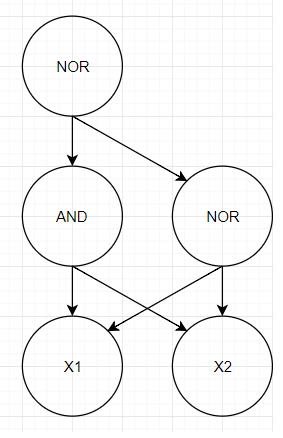
\includegraphics[scale=1]{xor.png}
		\caption{Example of grid that computes XOR}
		\label{xorex}
	\end{figure*}
	 This was run on a 3 by 3 grid with a population size of 200 and with 20 generations. The tournament size was 7, and the crossover probability was 0.7. Also, the probability for global, link, and node mutations were all set to be 0.25.  In Figure \ref{xor_scalability}, we show the scalability of the XOR program.

	\begin{figure*}
		\centering
		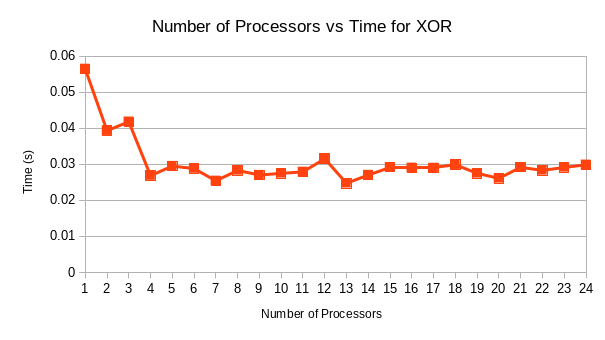
\includegraphics[width=\textwidth]{xor_scalability.png}
		\caption{Scalability of XOR}
		\label{xor_scalability}
	\end{figure*}

	Our program also successfully computed even-3 parity with different programs every run. In Figure \ref{parityex}, we show an example of a grid that computes even-3 parity.

	\begin{figure*}
		\centering
		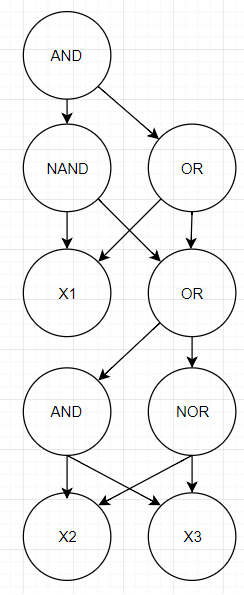
\includegraphics{parity1.png}
		\caption{Example of grid that computes even-3 parity}
		\label{parityex}
	\end{figure*}
	
	In Figure \ref{parity_scalability}, we show the scalability of the even-3 parity program. This was run on a 4 by 2 grid with a population size of 2000 and with 50 generations. The tournament size was 30, and the crossover probability was 0.7. Also, the probability for global, link, and node mutations were all set to be 0.05. Our program successfully discovers new ways to compute even-3 parity with every run.

\begin{figure*}
	\centering
	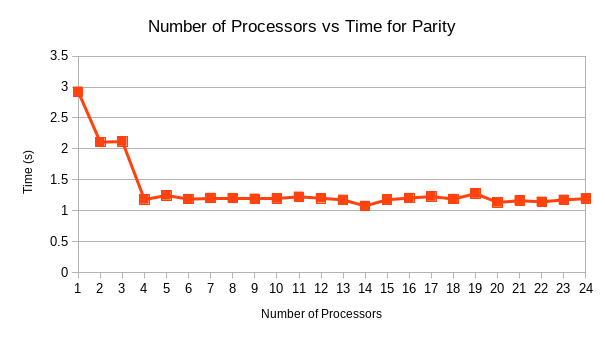
\includegraphics[width=\textwidth]{parity_scalability.png}
	\caption{Scalability of Even-3 Parity}
	\label{parity_scalability}
\end{figure*}
	
	\section{Future Work}
	
	Currently, our approach is restricted to be a feed-forward grid, and as such, we cannot expect to solve any problems that go beyond the scope of a general combinatorial circuit. Ideally, we want to compute general functions. One simple extension would be to compute symbolic regressions, in which our non-terminals would be common mathematical operators, and we would try to deduce what function maps a given set of training points. Another nice expansion would be to use assembly instructions as our non-terminals and have our input nodes accept some string encoding to our program.
	
	We also could try experimenting with different crossover operations. At the moment, we have one specific kind of crossover that truncates the subgraph if it is too large to fit in the other parent's grid. However, there are other variants that may handle these cases differently such as wrapping around the grid instead.
	
	Additionally, another way to generalize our approach would be to use meta-genetic programming \cite{b5}. Currently, we hard-code in the parameters to our prog
	rams for each example such as the crossover and mutation probabilities or tournament size. In theory, these parameters can also be evolved with our programs. However, it is not clear that this would add much benefit, but can be something to experiment with.
	
	\begin{thebibliography}{00}
				
		\bibitem{b1} McPhee, Nicholas Freitag, Riccardo Poli, and William B. Langdon. Field
		guide to genetic programming. (2008).
		
		\bibitem{b2} S.Handley. On the use of a directed acyclic graph to represent a population of computer programs. In Proceedings of the 1994 IEEE World Congress on Computational Intelligence, pages 154-159, Orlando, Florida, USA, 27-29 June 1994. IEEE Press.

		\bibitem{b3} Poli, Riccardo. Parallel distributed genetic programming. University of Birmingham, Cognitive Science Research Centre, 1996.

		\bibitem{b4} Kilian Stoffel and Lee Spector. High-performance, parallel, stack-based genetic programming. In John R. Koza, David E. Goldberg, David B. Fogel, and Rick L. Riolo, editors, Genetic Programming 1996: Proceedings of the First Annual Conference, page 224, Stanford University, CA, USA, 28-31 July 1996. MIT Press.
			
		\bibitem{b5} B. Edmonds, “Meta-genetic programming: Co-evolving the operators of variation,” CPM Report No.: 98-32. Centre for Policy Modelling, Manchester Metropolitan University. http://www.cpm.mmu.ac.uk/cpmrep32.html, 1998.
		\end{thebibliography}
	
\end{document}
